\documentclass{article}
\usepackage[utf8]{inputenc}
\usepackage{tabularx} % extra features for tabular environment
\usepackage{amsmath}  % improve math presentation
\usepackage{graphicx} % takes care of graphic including machinery
\usepackage{listings}
\usepackage{xcolor}

\definecolor{codegreen}{rgb}{0,0.6,0}
\definecolor{codegray}{rgb}{0.5,0.5,0.5}
\definecolor{codepurple}{rgb}{0.58,0,0.82}
\definecolor{backcolour}{rgb}{1, 1, 1}

\lstdefinestyle{mystyle}{
    backgroundcolor=\color{backcolour},   
    commentstyle=\color{codegreen},
    keywordstyle=\color{magenta},
    numberstyle=\tiny\color{codegray},
    stringstyle=\color{codepurple},
    basicstyle=\ttfamily\footnotesize,
    breakatwhitespace=false,         
    breaklines=true,                 
    captionpos=b,                    
    keepspaces=true,                      
    showspaces=false,                
    showstringspaces=false,
    showtabs=false,                  
    tabsize=2
}

\lstset{style=mystyle}

\usepackage{xspace}
\usepackage{multirow}
\usepackage{tikz}
\usepackage{enumitem}
\usetikzlibrary{babel}
\usepackage[american]{circuitikz}
\usetikzlibrary{calc}
\usepackage{siunitx}
\usepackage{pgfplots}
\usepackage[skins,theorems]{tcolorbox}
\tcbset{highlight math style={enhanced,
  colframe=red,colback=white,arc=0pt,boxrule=1pt}}
\pgfplotsset{width=10cm,compat=1.9}
\usepackage[margin=1in,letterpaper]{geometry} % decreases margins
\usepackage{cite} % takes care of citations
\usepackage[final]{hyperref} % adds hyper links inside the generated PDF file
\hypersetup{
colorlinks=true,       % false: boxed links; true: colored links
linkcolor=blue,        % color of internal links
citecolor=blue,        % color of links to bibliography
filecolor=magenta,     % color of file links
urlcolor=blue        
}
\begin{document}

\title{\textbf{Homework Assignment 2}}
\author{\textbf{TADIPATRI UDAY KIRAN REDDY}\\\textbf{EE19BTECH11038}}
\maketitle
\section{\textbf{MOSFET Resistance}}

\section{\textbf{MOSFET Capacitance}}
\textbf{Long channel TestBench}\\
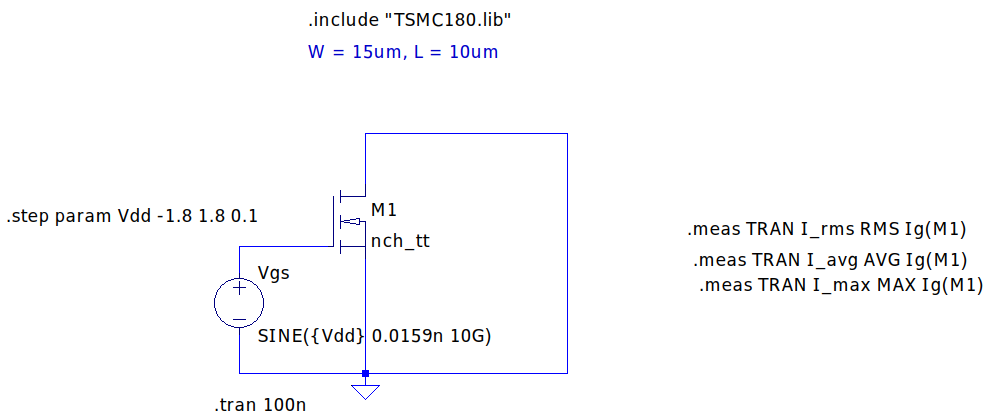
\includegraphics[scale=0.4]{./figs/Q2_nmos_lc_tb.png}\\
 \newline
\textbf{Short channel TestBench}\\
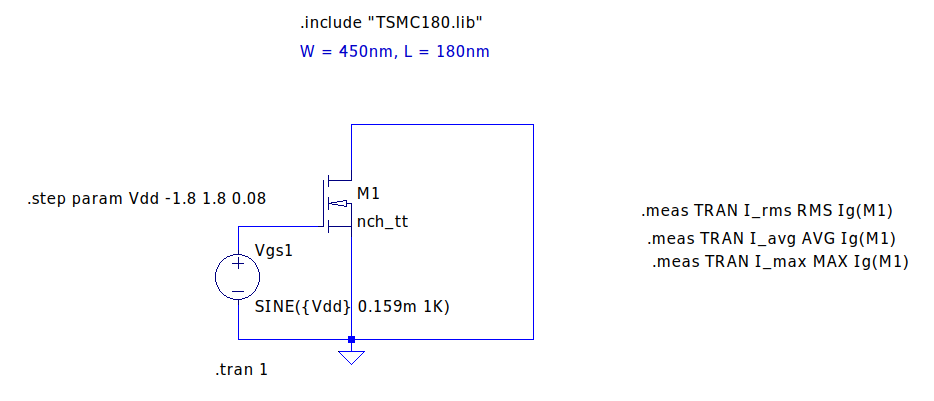
\includegraphics[scale=0.4]{./figs/Q2_nmos_sc_tb.png}\\
\subsection*{(a)}
This simulation was done @ 1KHz with AC amplitude of 0.159mV.\\
\textbf{Long Channel, W = 15$\mu$m L = 10$\mu$m}\\
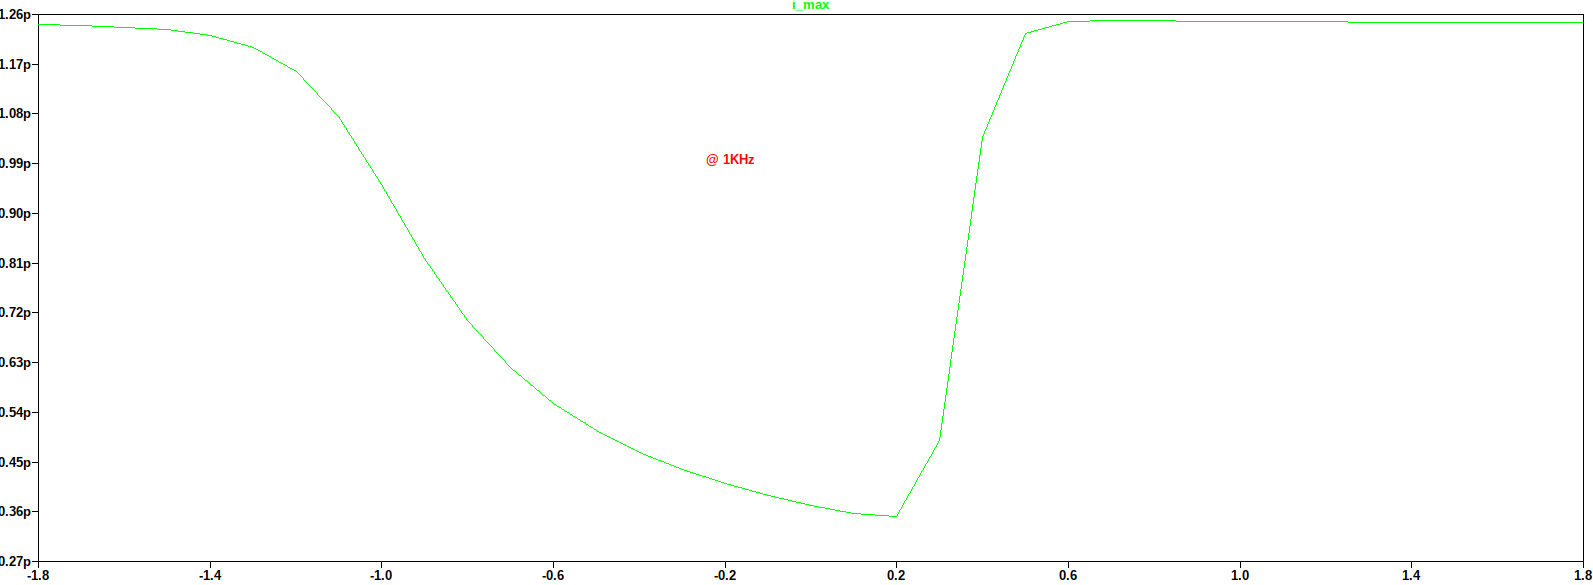
\includegraphics[scale=0.33]{./figs/Q2_nmos_lc_1K.png}\\
 \newline
\textbf{Short Channel, W = 450nm L = 180nm}\\
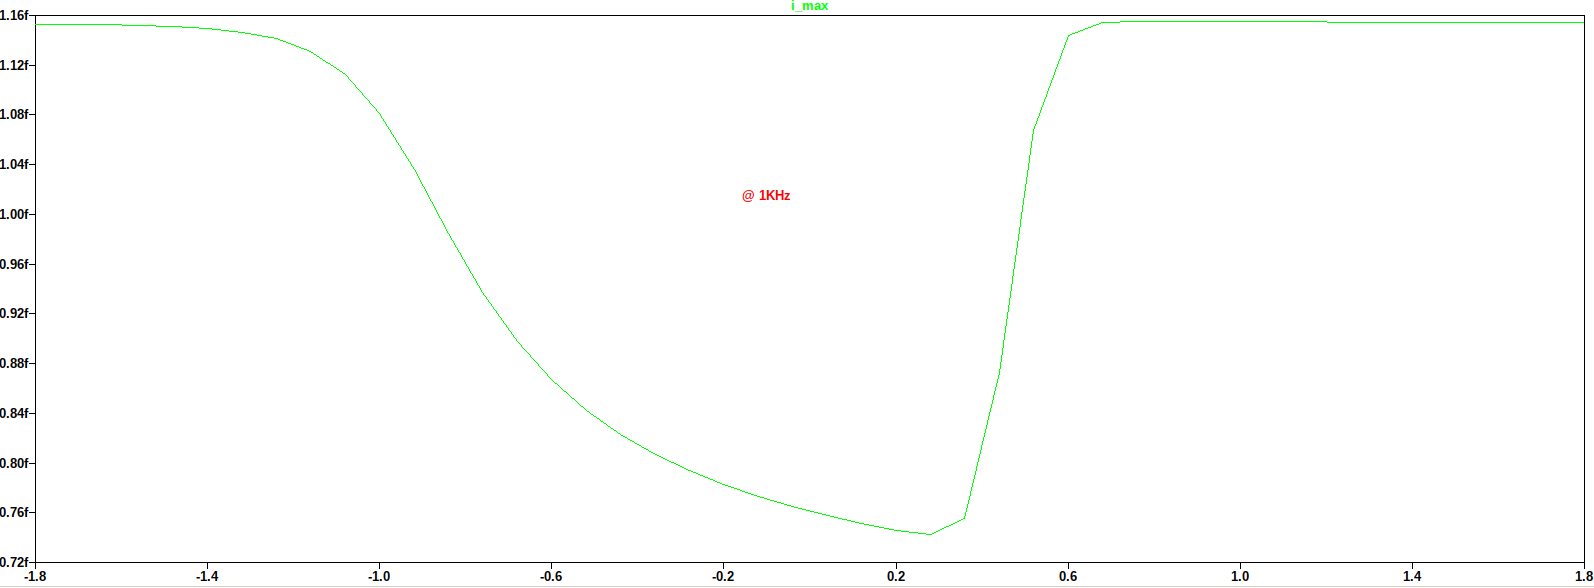
\includegraphics[scale=0.33]{./figs/Q2_nmos_sc_1K.png}\\
 \newline
The above simulation follow same trends as \textit{Figure 3.31(b) of Jon Rabaey}, We see that in both long and short channel the Capacitance observed to constant in regions when $V_{gs}$ is in range $[-1.8V, -1V] \bigcup [0.5V, 1.8V]$ and reduces from $[-1V, 0.2V]$ and increases in range of $[0.2V, 0.5V]$ in the case of Long channel, where as in Short channel reduces from $[-1V, 0.3V]$ and increases in range of $[0.3V, 0.5V]$.
\subsection*{(b)}
\textbf{Long Channel, W = 15$\mu$m L = 10$\mu$m}\\
\textbf{@ 10MHz}\\
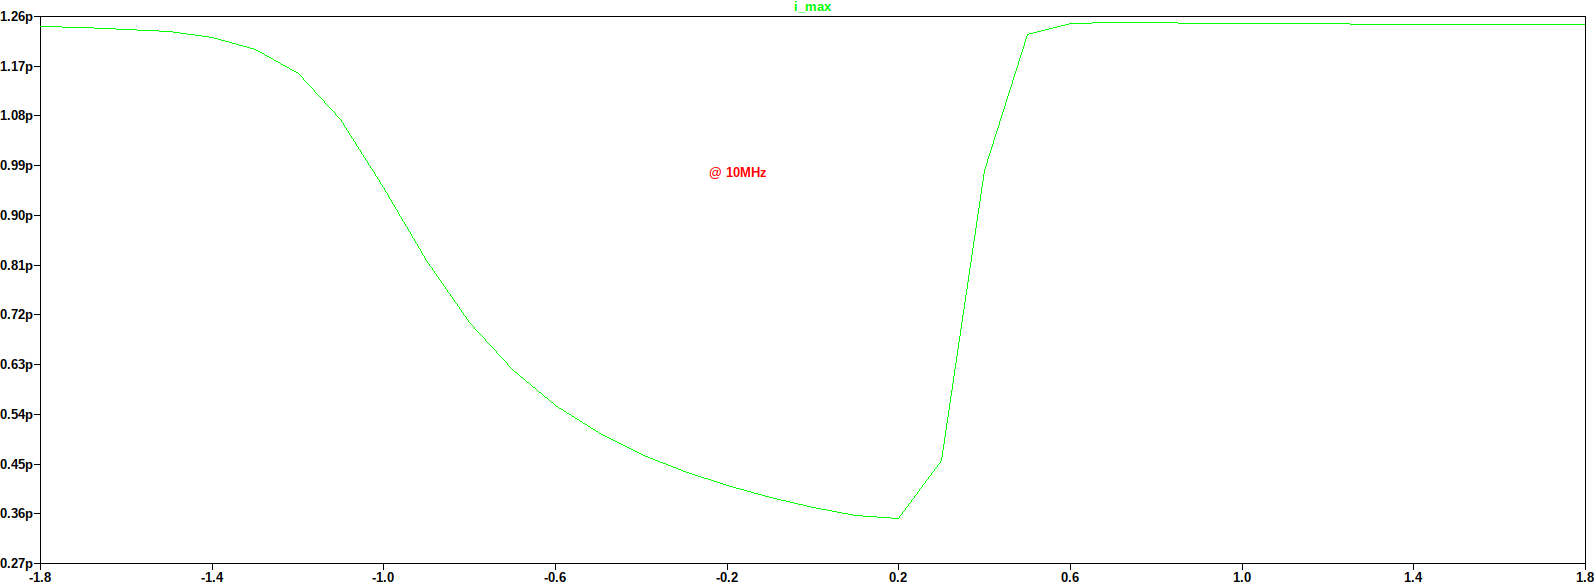
\includegraphics[scale=0.33]{./figs/Q2_nmos_lc_10M.png}\\
 \newline
\textbf{@ 10GHz}\\
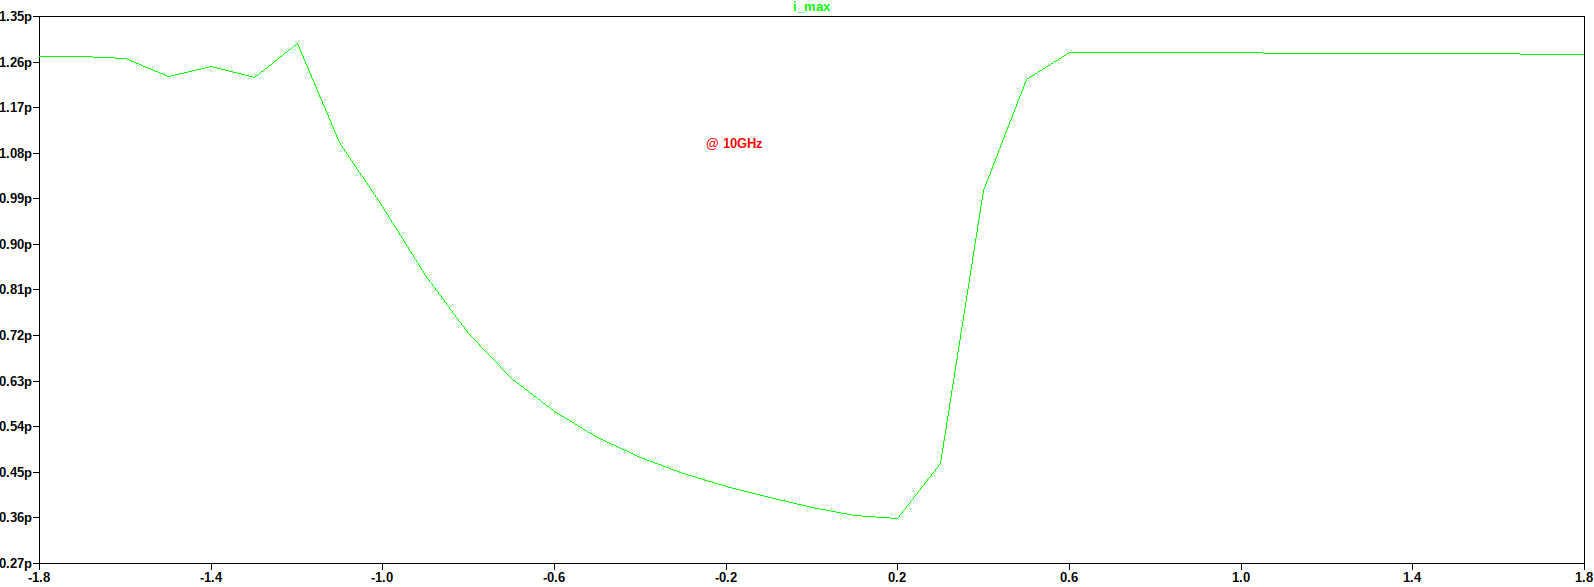
\includegraphics[scale=0.33]{./figs/Q2_nmos_lc_10G.png}\\
 \newline
\textbf{Short Channel, W = 15$\mu$m L = 10$\mu$m}\\
\textbf{@ 10MHz}\\
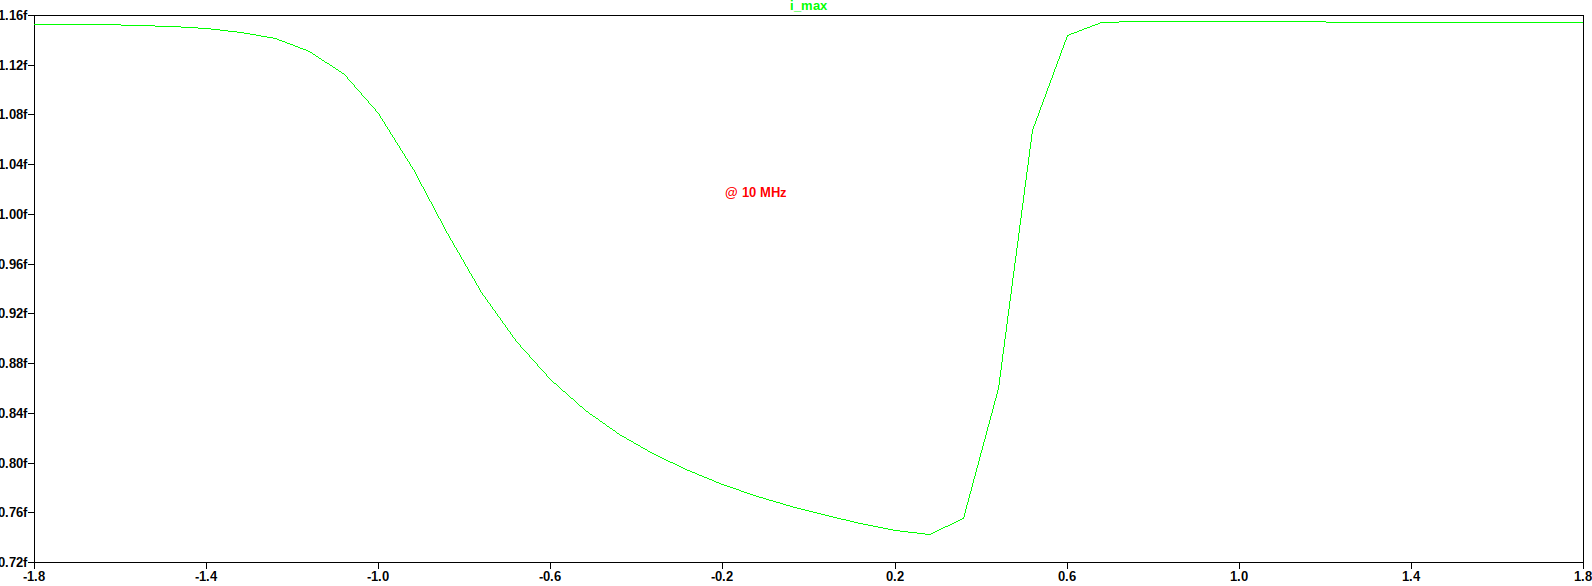
\includegraphics[scale=0.33]{./figs/Q2_nmos_sc_10M.png}\\
 \newline
\textbf{@ 10GHz}\\
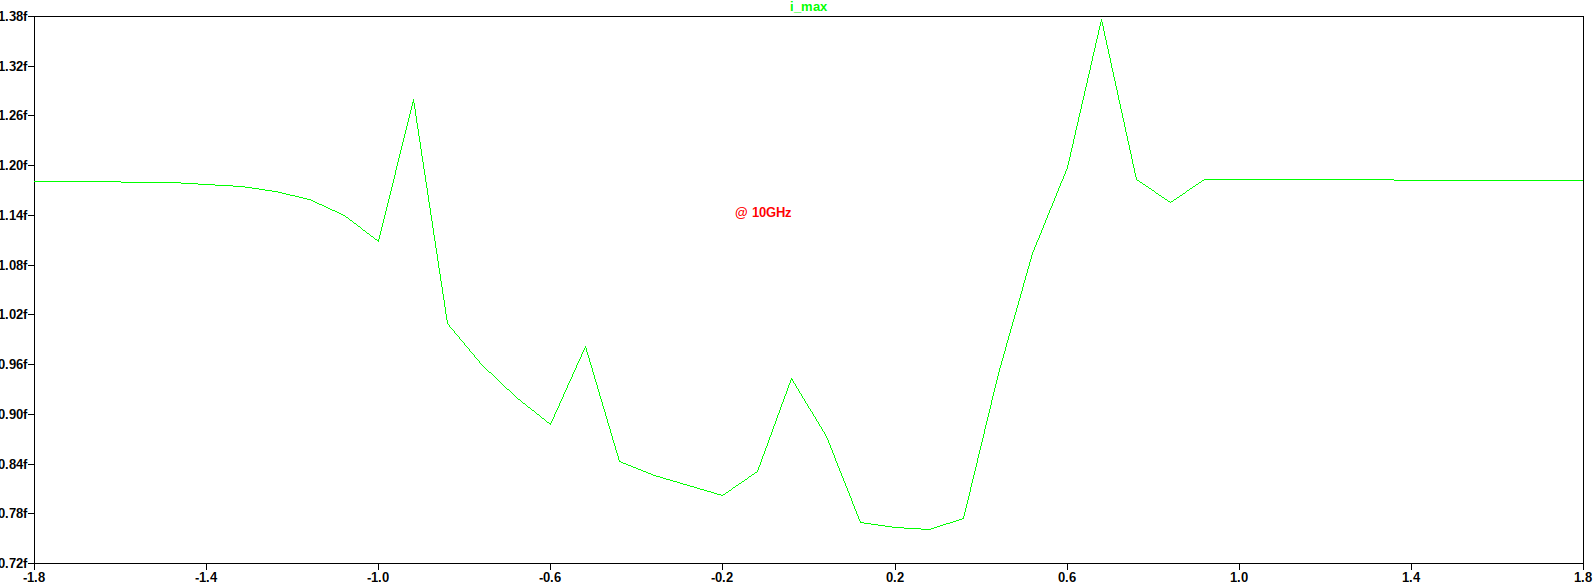
\includegraphics[scale=0.33]{./figs/Q2_nmos_sc_10G.png}\\
 \newline
In CV characteristics @ 10MHz and 10GHz we see that there is lot of bizzare behaviour, possible reasons can be due to high frequecncy behaviour of dieletic in mosfet affecting it's dielectric constant at high frequencies there by having bizzare capacitances.
\section{\textbf{Inverter Implementations}}
\subsection*{(a) Which one(s) of the circuits consume(s) static power when the input is high
($V_{IN}$ = 1.2 V )?}
\textbf{\textit{Circuit (i)}}\\
This consumes static power as when input is HIGH, output would be LOW thus making a potential differnce across resistaor and as NMOS is in triode region it also conducts thus there would be a constant current flow accounting for ohmic losses.\\
 \newline
\textbf{\textit{Circuit (ii)}}\\
NMOS above is self-biased mosfet which is in saturation as $V_{ds}$=1.2-$V_{out}$ and $V_{gs}$=1.2-$V_{out}$, clearly $V_{ds} > V_{gs} - V_T$. There by a constant DC current would flow through MOS creating ohmic losses.\\
 \newline
\textbf{\textit{Circuit (iii)}}\\
This is same case as that Circuit (ii) but here $V_{ds} = V_{gs} - V_T$, here also a DC current flows causing ohmic loss.

\subsection*{(b) Which one(s) of the circuits consume(s) static power when the input is low($V_{IN}$ =
0 V )?}
\textit{\textbf{None of these circuits will draw static power when INPUT is LOW.}}

\subsection*{(c) $V_{OH}$ of which circuit(s) is 1.2 V (if possible)?}
\textit{Circuit (i)}\\
If $V_{in}$ is zero, that means NMOS is in cut-off region thus no current flows. Now this effectively is a RC circuit while output voltage is the voltage accros capacitor given sufficient time the capacitor indeed charges to max value.\\
 \newline
\textit{Circuit (iii)}\\
In circuit(ii),upper NMOS is in saturation and when $V_{g}=V_{d}=1.2V$, the device cannot pass HIGH but has a drop of $V_{T}$. Whereas here in this circuit the gate has a voltage of 1.5 which is 1.2+0.3(=$V_T$). Thus here HIGH would pass without drop. There by this topology can pull HIGH.\\
 \newline
\textit{Circuit(iv)}\\
Clearly PMOS passes HIGH thus pulling up the output voltage to 1.2V.
\subsection*{(d) $V_{OL}$ of which circuit(s) is 0 V (if possible)?}
\textit{Circuit(i)}, \textit{Circuit(ii)}, \textit{Circuit(iii)} and \textit{Circuit(iv)}\\
All topologies have NMOS's drain as output and we know that NMOS is very good at passing LOW, there by pulls the output or discharges the output voltage to 0V.
\subsection*{(e) The proper functionality of which circuit(s) depends on the size of the devices?
(Note that they are designed for a digital inverter)}

\section{\textbf{NMOS Inverter - manual analysis}}
\begin{figure}[h]
\centering
\begin{circuitikz}[american]
\ctikzset{tripoles/mos style/arrows}
\ctikzset{tripoles/pmos style/nocircle}
\draw (0,-0.0) node[nmos](Q1){NMOS};\draw (Q1.D) to[short] (0,1.0);
\draw (Q1.S) to[short] (0,-1.0);
\draw (Q1.G) to[short] (-1,-0.0);
\draw (-1,-0.0) to[short] (-2,-0.0);
\draw (0,4.0) to[R,l=$R$, i=$i_{ds}$] (0,2.0);
\draw (0,-2.0) node[ground]{};
\draw (0,-2.0) to[short] (0,-1.0);
\draw (0,1.0) to[short] (0,2.0);
\draw (0,1.0) to[short] (1,1.0);
\draw (0,4.0) node[vcc]{Vdd};
\draw (1,1.0) node[vcc]{$V_{out}$};
\draw (-2,-0.0) node[vcc]{$V_{in}$};
\end{circuitikz}
\end{figure}
\textbf{Parameters},Taken from \textit{TSMC180.lib} file\\
${{\beta}_n}$ = 2*170.1$\mu$A/$V^2$\\
W/L = 1.5\\
$V_T$ = 0.4V\\
 \newline
Clearly,\\
\begin{equation*}
V_{out} = Vdd - i_{ds}R
\end{equation*}
And $i_{ds}$ depends on region on operation of the NMOS.\\
\textbf{Case(i) $V_{in} < V_T$, Cut-off region}\\
\begin{gather*}
i_{ds} = 0 \implies \tcbhighmath[drop fuzzy shadow]{V_{out} = Vdd}\\
\tcbhighmath[drop fuzzy shadow]{Gain = \frac{\partial V_{out}}{\partial V_{in}} = 0}
\end{gather*}
 \newline
\textbf{Case(ii) $V_{T} < V_{in} < V_{sl}$, Saturation region}\\
Where $V_{sl}$ is point where MOSFET changes its region of operation from saturation to triode region.\\
\begin{gather*}
i_{ds} = {{\beta}_n}{\frac{W}{2L}}(V_{in} - V_T)^2\\
\implies \tcbhighmath[drop fuzzy shadow]{V_{out} = Vdd - {{\beta}_n}{\frac{W}{2L}}R(V_{in} - V_T)^2}\\
@V_{in} = V_{sl}; V_{out} = V_{in} - V_T\\
\implies V_{in}-V_T = Vdd - {{\beta}_n}{\frac{W}{2L}}R(V_{in} - V_T)^2\\
V_{in} - V_T = \frac{-1 \pm \sqrt{1 + 2{{\beta}_n}{\frac{W}{L}}RVdd}}{{{\beta}_n}{\frac{W}{L}}R}\\
\implies \tcbhighmath[drop fuzzy shadow]{V_{sl} = V_T + \frac{\sqrt{1 + 2{{\beta}_n}{\frac{W}{L}}RVdd}-1}{{{\beta}_n}{\frac{W}{L}}R}}\\
\tcbhighmath[drop fuzzy shadow]{Gain = \frac{\partial V_{out}}{\partial V_{in}} = -{{\beta}_n}{\frac{W}{L}}R(V_{in}-V_T)}
\end{gather*}
 \newline
\textbf{Case(iii) $V_{in} > V_{sl}$, Triode region}\\
\begin{gather*}
i_{ds} = {{\beta}_n}{\frac{W}{L}}((V_{in} - V_T)^2V_{out} - \frac{{V^2}_{out}}{2})\\
\implies V_{out} = Vdd - {{\beta}_n}{\frac{W}{L}}R((V_{in} - V_T)^2V_{out} - \frac{{V^2}_{out}}{2})\\
V_{out} = \frac{\left(1 + {{\beta}_n}{\frac{W}{L}}R(V_{in} - V_T)\right) \pm \sqrt{\left(1 + {{\beta}_n}{\frac{W}{L}}R(V_{in} - V_T)\right)^2 - 2{{\beta}_n}{\frac{W}{L}}RVdd}}{{{\beta}_n}{\frac{W}{L}}R}
\end{gather*}
Intutively $V_{out}$ should decrease when $V_{in}$ increase thus we should take only the - case root, as its slope might be negative but in + case root the slope is always +ve there by increasing $V_{out}$ with $V_{in}$. This is contradiction with our assumption thus - case root is only possible solution.\\
\begin{gather*}
\tcbhighmath[drop fuzzy shadow]{V_{out} = \frac{\left(1 + {{\beta}_n}{\frac{W}{L}}R(V_{in} - V_T)\right) - \sqrt{\left(1 + {{\beta}_n}{\frac{W}{L}}R(V_{in} - V_T)\right)^2 - 2{{\beta}_n}{\frac{W}{L}}RVdd}}{{{\beta}_n}{\frac{W}{L}}R}}\\
\implies \tcbhighmath[drop fuzzy shadow]{Gain = \frac{\partial V_{out}}{\partial V_{in}} = 1 - \frac{\left(1 + {{\beta}_n}{\frac{W}{L}}R(V_{in} - V_T)\right)}{\sqrt{\left(1 + {{\beta}_n}{\frac{W}{L}}R(V_{in} - V_T)\right)^2 - 2{{\beta}_n}{\frac{W}{L}}RVdd}}}
\end{gather*}
Finally puting everything in a compact form we get,\\
\begin{gather}
V_{out} = \begin{cases}
	Vdd & V_{in} < V_T\\
	Vdd - {{\beta}_n}{\frac{W}{2L}}R(V_{in} - V_T)^2 & V_T < V_{in} < V_{sl}\\
	V_{out} = \frac{\left(1 + {{\beta}_n}{\frac{W}{L}}R(V_{in} - V_T)\right) - \sqrt{\left(1 + {{\beta}_n}{\frac{W}{L}}R(V_{in} - V_T)\right)^2 - 2{{\beta}_n}{\frac{W}{L}}RVdd}}{{{\beta}_n}{\frac{W}{L}}R} & V_{in} > V_{sl}
\end{cases} \label{eq:vout}\\
Gain = \frac{\partial V_{out}}{\partial V_{in}} = \begin{cases}
0 & V_{in} < V_T\\
-{{\beta}_n}{\frac{W}{L}}R(V_{in}-V_T) & V_{T} < V_{in} < V_{sl}\\
1 - \frac{\left(1 + {{\beta}_n}{\frac{W}{L}}R(V_{in} - V_T)\right)}{\sqrt{\left(1 + {{\beta}_n}{\frac{W}{L}}R(V_{in} - V_T)\right)^2 - 2{{\beta}_n}{\frac{W}{L}}RVdd}} & V_{in} > V_{sl}
\end{cases} \label{eq:gain}
\end{gather}
Where,
\begin{equation} \label{eq:vsl}
{V_{sl} = V_T + \frac{\sqrt{1 + 2{{\beta}_n}{\frac{W}{L}}RVdd}-1}{{{\beta}_n}{\frac{W}{L}}R}}
\end{equation}

\subsection*{(a)}
Switching threshould is when $V_{in} = V_{out} = V_{M}$, clearly this intersection point occurs only in saturation region.
\begin{gather*}
V_{M} = Vdd - {{\beta}_n}{\frac{W}{2L}}R(V_{M} - V_T)^2
\implies V_{M} = V_T + \frac{-1 \pm \sqrt{1 + 2{{\beta}_n}{\frac{W}{L}}R(Vdd-V_T)}}{{{\beta}_n}{\frac{W}{L}}R}\\
\end{gather*}
Since voltage always is positive
\begin{equation} \label{eq:vm}
V_{M} = V_T + \frac{\sqrt{1 + 2{{\beta}_n}{\frac{W}{L}}R(Vdd-V_T)}-1}{{{\beta}_n}{\frac{W}{L}}R}
\end{equation}
Using the specification of device, we get \textbf{$V_M$ = 706mV}.\\
 \newline
$V_{OH}$ and $V_{OL}$ are output voltages when Gain=-1. One point occurus in Saturation and other in Triode.\\
\textbf{Case(i) In Saturation region},\\
\begin{gather*}
-1 = -{{\beta}_n}{\frac{W}{L}}R(V_{IL}-V_T)
\end{gather*}
\begin{equation} \label{eq:vil}
\implies V_{IL} = V_T + \frac{1}{{{\beta}_n}{\frac{W}{L}}R}
\end{equation}
Then corresponding $V_{OH}$ is,
\begin{gather*}
V_{OH} = Vdd - {{\beta}_n}{\frac{W}{2L}}R(V_{IL} - V_T)^2
\end{gather*}
\begin{equation} \label{eq:voh}
	V_{OH} = Vdd - \frac{1}{2{{\beta}_n}{\frac{W}{L}}R}
\end{equation}
Then \textbf{$V_{OH}$ is 2.487V}.\\
 \newline
\textbf{Case(ii) In Triode region},\\
\begin{gather*}
-1 = 1 - \frac{\left(1 + {{\beta}_n}{\frac{W}{L}}R(V_{IH} - V_T)\right)}{\sqrt{\left(1 + {{\beta}_n}{\frac{W}{L}}R(V_{IH} - V_T)\right)^2 - 2{{\beta}_n}{\frac{W}{L}}RVdd}}\\
\implies \frac{\sqrt{\left(1 + {{\beta}_n}{\frac{W}{L}}R(V_{IH} - V_T)\right)^2 - 2{{\beta}_n}{\frac{W}{L}}RVdd}}{\left(1 + {{\beta}_n}{\frac{W}{L}}R(V_{IH} - V_T)\right)} = 2
\end{gather*}
Solving the above quadratic equation we get,
\begin{equation} \label{eq:vih}
	V_{IH} = V_T + 2\sqrt{\frac{2Vdd}{3{{\beta}_n}{\frac{W}{L}}R}} - \frac{1}{{{\beta}_n}{\frac{W}{L}}R}
\end{equation}
Then corresponding $V_{OL}$ is,
\begin{gather*}
V_{OL} = \frac{\left(1 + {{\beta}_n}{\frac{W}{L}}R(V_{IH} - V_T)\right) - \sqrt{\left(1 + {{\beta}_n}{\frac{W}{L}}R(V_{IH} - V_T)\right)^2 - 2{{\beta}_n}{\frac{W}{L}}RVdd}}{{{\beta}_n}{\frac{W}{L}}R} \\
V_{OL} = \frac{\left(1 + {{\beta}_n}{\frac{W}{L}}R(V_T + 2\sqrt{\frac{2Vdd}{3{{\beta}_n}{\frac{W}{L}}R}} - \frac{1}{{{\beta}_n}{\frac{W}{L}}R} - V_T)\right) - \sqrt{\left(1 + {{\beta}_n}{\frac{W}{L}}R(V_T + 2\sqrt{\frac{2Vdd}{3{{\beta}_n}{\frac{W}{L}}R}} - \frac{1}{{{\beta}_n}{\frac{W}{L}}R} - V_T)\right)^2 - 2{{\beta}_n}{\frac{W}{L}}RVdd}}{{{\beta}_n}{\frac{W}{L}}R}
\end{gather*}
\begin{equation} \label{eq:vol}
\implies V_{OL} = \sqrt{\frac{2Vdd}{3{{\beta}_n}{\frac{W}{L}}R}}
\end{equation}
Plugging the specification in to the above equation we get, \textbf{$V_{OL}$ as 209mV}.

\subsection*{(b)}
$V_{IL}$ and $V_{IH}$ are determined in equation \eqref{eq:vil} and \eqref{eq:vih} respectively.\\
Therefore Noise margins are obtained from equations \eqref{eq:vil}, \eqref{eq:vih}, \eqref{eq:vol} and \eqref{eq:voh},
\begin{gather*}
	NM_L = V_{IL} - V_{OL}
\end{gather*}
\begin{equation} \label{eq:nml}
	NM_L = V_T + \frac{1}{{{\beta}_n}{\frac{W}{L}}R} - \sqrt{\frac{2Vdd}{3{{\beta}_n}{\frac{W}{L}}R}}
\end{equation}
Similary for $NM_H$
\begin{gather*}
	NM_H = V_{IH} - V_{OH}
\end{gather*}
\begin{equation} \label{eq:nmh}
	NM_H = V_T - Vdd + 2\sqrt{\frac{2Vdd}{3{{\beta}_n}{\frac{W}{L}}R}} - \frac{1}{2{{\beta}_n}{\frac{W}{L}}R}
\end{equation}
Plugging the specs in the above equations we get, \textbf{$NM_L$ as 217mV} and \textbf{$NM_H$ as -1.696V}.

\subsection*{(c)}
Peak gain occurs only when NMOS, swicthes from saturation to triode, as in saturaion the gain is linear and decreases with increase in $V_{in}$. And in triode region the gain increases with increase with $V_{in}$. Therefore, Gain@$V_{in}=V_{sl}$ is maximum(speaking in absolute terms).\\
Then from equation \eqref{eq:vsl} we get,
\begin{gather*}
gain_{max} = -{{\beta}_n}{\frac{W}{L}}R(V_{sl}-V_T)
\end{gather*}
\begin{equation} \label{eq:gmax}
\implies gain_{max} = 1 -\sqrt{1 + 2{{\beta}_n}{\frac{W}{L}}RVdd}
\end{equation}
For this device we get, \textbf{$gain_{max}$ as -12.869}.
\section{\textbf{MOS Inverter- SPICE simulations}}
\begin{center}
\begin{tabular}{|c|c|c|c|}
\hline
\textbf{Parameter} & \textbf{Simulated} & \textbf{Calculated} & \textbf{Error(in \%)}\\
\hline
$V_{M}$ & 709.162mV & 706mV & -0.446\%\\
\hline
$V_{IL}$ & 409.587mV & 426mV & -4\%\\
\hline
$V_{HL}$ & 818.226mV & 791mV & -3.327\%\\
\hline
$V_{OL}$ & 159.3742mV & 209mV & \textbf{31.13\%}\\
\hline
$V_{OH}$ & 2.454V & 2.487V & 1.345\%\\
\hline
$NM_L$ & 250.2128mV & 217mV & \textbf{-13.27\%}\\
\hline
$NM_H$ & -1.63577V & -1.696V & 3.68\%\\
\hline
Peak gain & -8.758 & -12.869 & \textbf{46.9\%}\\
\hline
\end{tabular}
\end{center}
\end{document}
